\documentclass{article}

% if you need to pass options to natbib, use, e.g.:
% \PassOptionsToPackage{numbers, compress}{natbib}
% before loading nips_2017
%
% to avoid loading the natbib package, add option nonatbib:
% \usepackage[nonatbib]{nips_2017}

\usepackage{nips_2017}

% to compile a camera-ready version, add the [final] option, e.g.:
% \usepackage[final]{nips_2017}

\usepackage[utf8]{inputenc} % allow utf-8 input
\usepackage[T1]{fontenc}    % use 8-bit T1 fonts
\usepackage{hyperref}       % hyperlinks
\usepackage{url}            % simple URL typesetting
\usepackage{booktabs}       % professional-quality tables
\usepackage{amsfonts}       % blackboard math symbols
\usepackage{nicefrac}       % compact symbols for 1/2, etc.
\usepackage{microtype}      % microtypography
\usepackage[pdftex]{graphicx}
\usepackage{subfigure}
\usepackage{wrapfig}

\title{Lat-Net: Compressing Lattice Boltzmann Flow Simulations using Deep Neural Networks}

% The \author macro works with any number of authors. There are two
% commands used to separate the names and addresses of multiple
% authors: \And and \AND.
%
% Using \And between authors leaves it to LaTeX to determine where to
% break the lines. Using \AND forces a line break at that point. So,
% if LaTeX puts 3 of 4 authors names on the first line, and the last
% on the second line, try using \AND instead of \And before the third
% author name.

\author{
  Oliver Hennigh \\
  Mexico \\
  \texttt{loliverhennigh101@gmail.com} \\
}

\begin{document}
% \nipsfinalcopy is no longer used

\maketitle

\begin{abstract}
Computational Fluid Dynamics (CFD) is a hugely important field with applications in almost every engineering field, however, fluid simulations are extremely computationally and memory demanding. Towards this end, we present Lat-Net, a method for compressing both the computation time and memory usage of Lattice Boltzmann flow simulations using deep neural networks. Lat-Net employs convolutional autoencoders and residual connections in a fully differentiable scheme to compress the state size of a simulation and learn the dynamics on this compressed form. The result is a small computationally and memory efficient neural network that can be iterated and queried to reproduce a fluid simulation. We show that once Lat-Net is trained, it can generalize to large grid sizes and complex geometries while maintaining accuracy. We also show that Lat-Net is a general method for compressing other Lattice Boltzmann based simulations such as Electromagnetism.

\end{abstract}

\section{Introduction}

Computational fluid dynamics (CFD) is a branch of fluid dynamics that deals with numerically solving and analyzing fluid flow problems such as those found in aerodynamics, geology, biology, etc. CFD simulations are known for their high computational requirements, memory usage, and run times. Becuase of this, there is an ever growing body of work using simulation data to create reduced order models that can be evaluated with sigificantly less resources. Towards this end, we develop a neural network approach that both compresses the computation time and memory usage of fluid simulations.

We investigate fluid simulations that contain complex time dependent turbulence. Simulations of this form are difficult because they require fluid solver to have high resolution and small times steps. Never the less, they frequently occur in nature and are an imporant area of study. Motivated by need for these simulations and the recent suscess of neural network based suraget models in related areas \cite{tompson2016accelerating} \cite{guo2016convolutional}, we choice this setting to test our model.

The most popular approach to modeling fluid flow is with the Navier stokes equation. The solution to this partial differential equation gives the flow velocity field for a given domain. Recently, there has been a new method for simulating fluid flow named the Lattice Boltzmann Method (LBM). It is derived from the boltzmann equation and grew out of Lattice Gas Automaton (LGA) in the late 80s \cite{mcnamara1988use}. The main advantages of LBM are its ability to run on complex geometrys, its scalability to parallel architectures and applicability to complex flows that contain phemomena such as heat transfer and chemical reactions. For these reasons, there has been much development in the area. Because of this methods popularity and techinqual details we will discuss later, our approach is centered around this method of simulation.

Our proposed method works by compressing state of the simulation while learning the dynamics of the simulation on these compressed forms. The model can be broken up into three pieces, an encoder, compression mapping, and decoder. The encoder compresses the both the state of the simulation as well as the given boundary conditions. The compression mapping learn dynamics on the compressed state that corrispond to the dynamics in the fluid simulation. The decoder decompresses the compressed state allowing for either the whole simulation state or desired pieces to extracted.

We focus the content of this paper on LBM Fluid Simulations because this is the most popular use of the LBM however this method is known to be a general partial differential equation solver (of a particular form cite em paper). LBM can in fact be used to solve many physical systems of interest such as Electormagnatism, Plasma, Multiphase flow, Schordiener equation etc \cite{mendoza2010three} \cite{kim2008wavelet} \cite{zhong2006lattice} \cite{shan1993lattice}. With this in mind, we keep our method general and show evidence our method works equaly effectively on Electromagnatism simulations. However, Because the domanate use of LBM is on fluid flow problems we center discustion on this subject with only minor look at other problems

Our method has several key contributions over other work applying neural networks to fluid simulations. Bellow is a list our key contributions.
\begin{itemize}
  \item It allows for simulations to be generated with less memory then the original flow solver. There is a crucial need for such methods because memory requirements grow cubic to grid size in 3D simulations. In practice, this quickly results in the need for large GPU clusters \cite{onodera2013large} \cite{xian2011multi}.
  \item Once our model is trained, it can be used to generate significantly larger simulations. This allows the model to learn from a training set of small simulations and then generate simulations as much as 16 times bigger with little effect in accuracy.
  \item Our method is directly applicable to a variety of physics simulations, not just fluid flow. We show this with our electromagnetic example and note that the changes to our model to acomidate any Lattice Boltzmann type simulation are trivial.
\end{itemize}

\section{Related Work}

Recently, there have been several papers applying neural network to fluid flow problems. Guo etc \cite{guo2016convolutional} proposed to use a neural network to learn a mapping from the boundary conditions to the steady state flow. In \cite{yang2016data} blaa. Most related to our own work, Tompson ect. \cite{tompson2016accelerating} uses a network to solve the Poisson equation to accelerate eulerian fluid simulations. The key difference between this and Lat-Net is its ability to compresse the memory of the simulation and the generability of our method to other physics simulations.

There has also been an increasing body of work applying neural networks to other physics modeling problems. For example, neural networks have been readly addopted in many chemisty aplications such as predicting molecular properties from descriptors, protein contact prediction and computational material design \cite{goh2017deep}. Very recently, neural networks have been applied to quantum mechanics problems as seen in Mills ect \cite{mills2017deep} and Giuseppe ect \cite{carleo2017solving} where neural networks are used to approximate solutions to the schodiener equation. In Paganini etc \cite{2017arXiv170502355P}, they use generative advesarial networks \cite{goodfellow2014generative} to model electromagnetic showers in a longitudinally segmented calorimeter. Many of these applications are relatively recent and indecate a resurgance of interest in applications of neural networks to modeling physics.

Reduced order Modeling is an area of research that focuses on techniques to reduce the dimentionality and computational complexity of mathematical models. A Reduced order model (ROM) is constructed from high-fidelity simulations and can subsequently be used to generate simulations for lower computation. The most popular ROM method for fluid dynamics is Galerikin projection \cite{barone2009reduced}. This method uses Proper Orthogonal Decomposition to reduce the dimenstionality of flow simulations and then finds the dynamics on this reduced space.  
While these approaches are centered around the navier stokes equation and thus not directly comparible to our own, we note that the compression mapping present in these methods is typicaly a linear projection or clustering. Given the recent success neural networks have had over these methods in creating well structured encodings (such as Variational Autoencoders \cite{kingma2013auto} \cite{watter2015embed}), we feel our approach is well justified.

\section{Deep Neural Networks for Compressed Lattice Boltzmann}

In this section, we present our model for compressing Lattice Bolztmann simulations.

\subsection{Review: The Lattice Boltzmann Method}

\begin{figure}[!t]
\centering
\subfigure{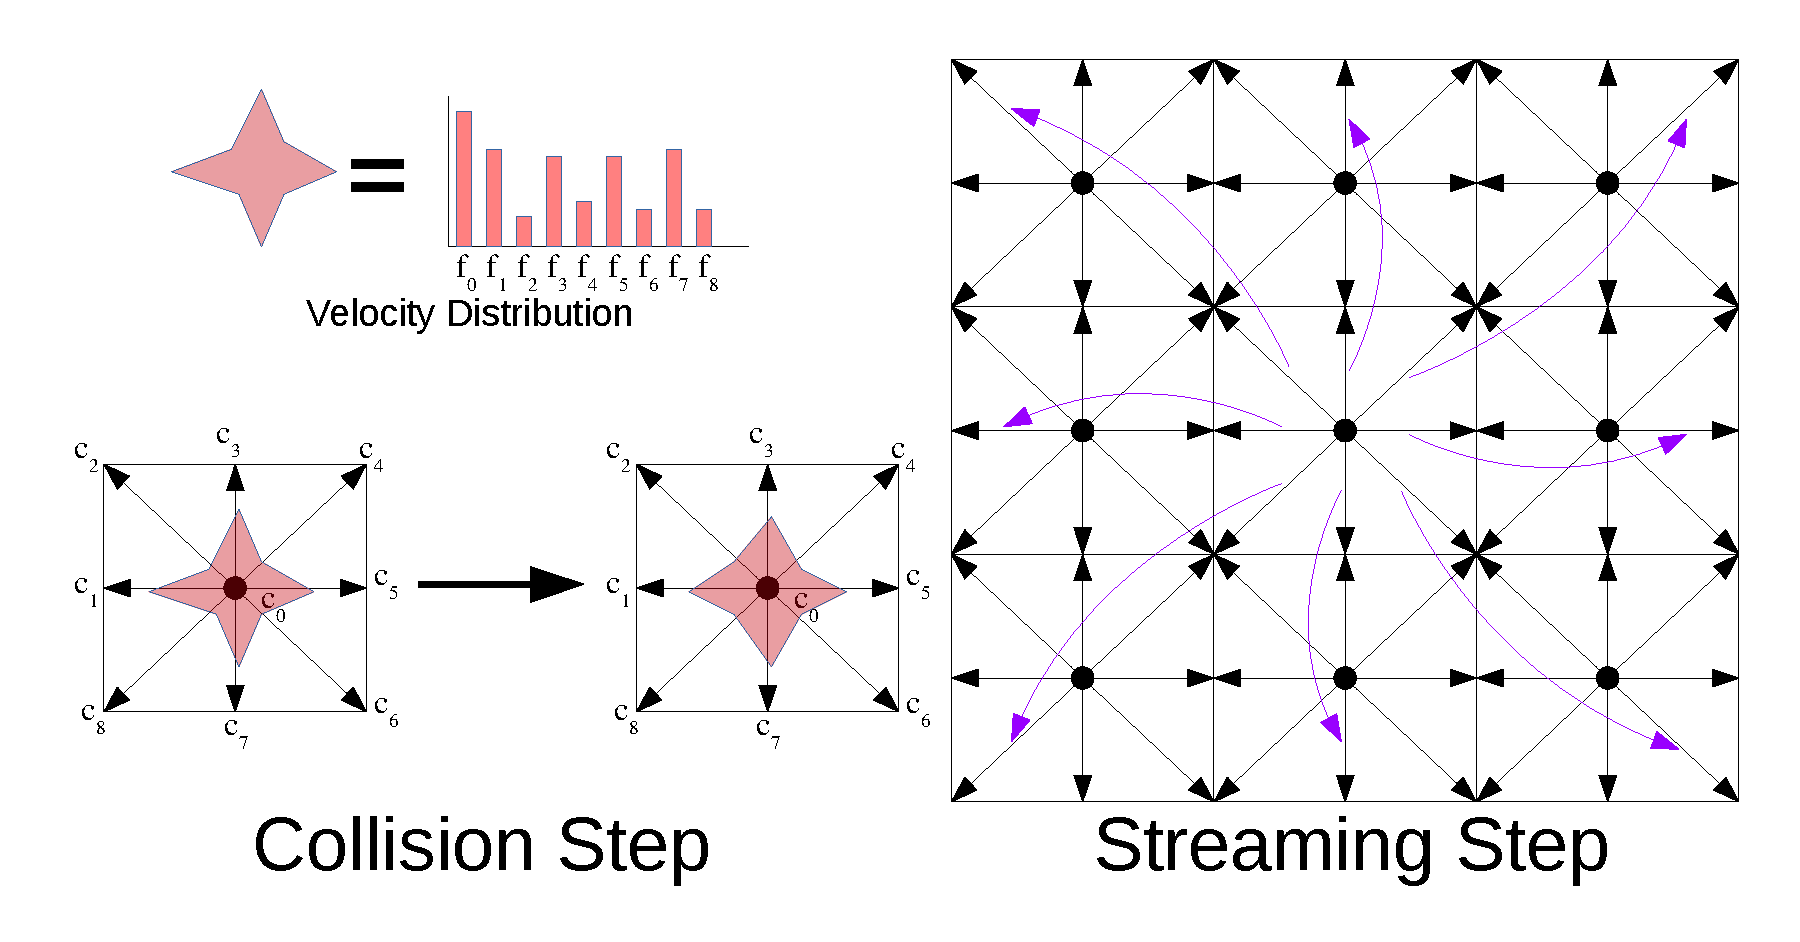
\includegraphics[scale=0.2]{../test/figs/lattice_boltzmann.pdf}}
\caption{Illustion of the Lattice Boltzmann update steps}
\label{lattice_boltzmann}
\end{figure}

In Lattice Boltzmann simulation, the domain is discrited into an equal sized Cartesian grid. Each cell of this grid contains a velocity ditrobution function $f_i$ that corrisponds to the velocity of the flow at that point. $f_i$ has $i$ possible direction of flow in the directions $\{ \vec{c}_i \}$. In our 2 dimentional simulations, there are 9 diffrent directions of flow. A figure showing this grid structur is seen in \ref{lattice_boltzmann}. From the distrobution function $f_i$, one can calculate the density ($p$) and velocity ($\vec{u}$) of the fluid flow with the following equations.

\begin{equation}
  p = \sum_i f_i  \qquad\text{and}\qquad \vec{u} = \sum_i \vec{c}_i f_i 
\end{equation}

The lattice states are updated with two seperate steps, the collision step and the streaming step. The collision step mimics the flow interacting with itself and is updated in the following way,

\begin{equation}
  f^t_i(x, t + \delta_t) = f_i(x,t) + \frac{1}{\tau} (f_i^{eq} - f_i)
\end{equation}

where $\tau$ is the relaxation constant and $f_i^{eq}$ is the flow equilibrium. For our simulations, we use the $f_i^{eq}$ from the Lattice Bhatnagar-Gros-Krook (LBGK) scheme. After the collition step is applied, the flow propegates to ajacent cells following the streaming step. 

\begin{equation}
  f_i(x + c_i, t + \delta_t) = f^t_i(x,t + \delta_t)
\end{equation}

Figure \ref{lattice_boltzmann} illustrates these steps for the 2 dimensional case. These steps are applied 

The important aspect of the LBM for our purposes is that it acts localy on grid cells. The area of effect a cell is directly proporitional to the number of applications of the evolution equation. This means that in $n$ time steps a cells value can be determinied exaclty with only the infomation of the cells within $n$ distance. This is important to know for our purposes becasue if we expect to treat the lattice boltzmann simulation as deterministic we must make sure our model 

\subsection{Proposed Architecture}

Figure \ref{fig_1} shows a sketch of the model. The figure can be understood by following the arrows starting from the flow state $f_t$ and the boundary $b$. Bellow we walk through each step of our method.

First, the network compresses both the state of the fluid simulation $f_t$ and a binary representation of the boundary conditions $b$ using two separate neural networks $\phi_{enc}$ and $\phi'_{enc}$ respectively. The result from $\phi_{enc}$ is a compressed representation of the flow $g_t$ and the result of $\phi'_{enc}$ are two tensors $b_{mul}$ and $b_{add}$ of equal size to $g_t$. These three tensors represent the entirety of the compressed state of the simulation.

In a Lattice Boltzmann solver, the boundary conditions are used at each timestep to add collision to the streaming step. In a similar way, our model applies the compressed boundary conditions to the compressed state every timestep. We do this in the following way,
\begin{equation}
  g_t = (g_t \odot b_{mul}) + b_{add}
\end{equation}
This method has proved extremely successful at keeping the boundary information firmly planted through the duration of the simulation. This method of applying boundary conditions was inspired by \cite{vondrick2016generating} where they use a similar method to combine foreground and background information in video prediction. After the boundary is applied to $g_t$, we can run the state through another neural network to emulate the dynamics, ie. $\phi_{comp}:g_{t} \rightarrow g_{t+1}$. Each step of $\phi_{comp}$ is equivalent to $n$ time step of the Lattice Boltzmann solver. For example, in the 2 dimensional simulation, each step of $\phi_{comp}$ represents 120 steps of the Lattice Boltzmann solver. Once $g_t$ is computed, we can extract out the generated state of the simulation with a decoder network $\phi_{dec}$. 

\begin{figure}[!t]
\centering
\subfigure{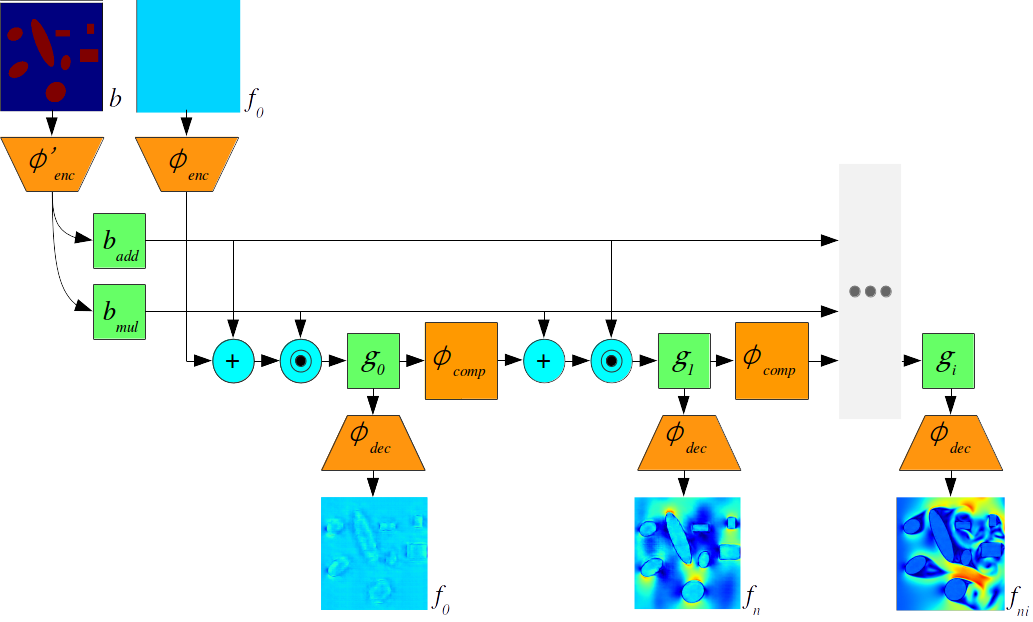
\includegraphics[scale=0.3]{../test/figs/fig_1.pdf}}
\caption{Illustration of the Lat-Net architecture}
\label{fig_1}
\end{figure}

\subsection{Network Implementation Details}

We implement 2 networks trained on 2 dimensional and 3 dimensional lattice simulations. The encoder, compression mapping and decoder pieces of the 2D network are each a series of 3x3 residual blocks in the sequences 4x(down res, res), 4x(res), and 4x(res, up res), respectively \cite{he2016deep}. For the 3D network, the sequences are 2x(down res), 3x(res), and 3x(up res) where 3x3x3 convolutions. The up and down residual blocks are created by replacing the first convolution with a 

Down sampling is produced by 4 by 4 convolutions with stride 2. Some of the simulations trained on have periodic boundary conditions. In these cases, we pad the appropriate edges periodicity before the convolution operations.

As mentioned above, each network is kept entirely convolutional. Fluid flow is inherently spatially correlated so using convlutional layers allows this spatial information to be preserved. Keeping the network convolutional also allows different input sizes to be used. This is how our model is able to train on small simulations and then generate larger simulations. During the course of this work, fully connected layers were explored however they produced extremely poor results.

Residual connections have been used in many deep learning architectures with much success. Adding residual connections allows for much deeper networks to be trained often resulting in improved results \cite{he2016deep}. When training our model, it is necessary to unroll the compression network over several time steps. This has the same effect as making the network deeper. For this reason, it seems logical to take advantage of this network architecture. We have seen that removing these residual connections results in much slower convergence and worse accuracy.

\subsection{Training Details}

Lat-Net is trained by unrolling the network and comparing the generated flow with the true. Our loss function is simply Mean Squared Error (MSE) although various loss functions were attempted throughout this work such as Image Gradient Difference Loss (GDL) \cite{mathieu2015deep}.  

Lat-Net is trained with the Adam optimizer \cite{kingma2014adam}.

\section{Experiments}

In this section we descirbe our experiments testing Lat-Net on a variety of problems. Our experiments are designed to tests our models ability to generate large simulation as well as its transferability to new datasets. We also explore computaitonal speed increase and trade off between memory compression and error. Finaly, we breifly show results applying this method to electromagnetic simulations.

\subsection{Dataset Generation}
In order to train and test our model, we generated sets of fluid and electromagnetic simulations. All simulations were generated with the MechSys library (find citation).

The train set for the 2 dimensional fluid simulation are grid size 256 by 256 and use 9 directional flows in the lattice boltzmann solver (D2Q9 scheme)\cite{guo2013lattice}. The simulation used periocid boundary conditions on top and bottom as well as uniform inlet flow and outlet flow of 0.04 from the left and right. 8 Objects are placed randomly with height and width sizes rangeing from 140 to 20 cells. The test set for the 2 dimesional simulations are of size 256 by 256, and 1024 by 1024 with the same boundary conditions and object densitys. We also generate a test set of size 256 by 512 with vehical cross sections as objects. There are 28 cross sections used ranging from trucks to minivans. For all 2 dimensional simulations, the ratio of network steps to lattice boltmann steps is 1 to 120.

The train set for the 3 dimensional fluid simulations are grid size 40 by 40 by 160 and use 15 directional flows in the lattice boltzmann solver (D3Q15 scheme)\cite{guo2013lattice}. Similar to the 2d simulations, periodic boundary conditions are used with same inlet and outlet flow. 4 spheres are randomly placed with height and width 24. The reason different object geometrys and sizes were not explored was due to the fact that smaller objects or objects with complex geometries tended to have too course a resolution for the lattice boltzmann solver and larger objects required too large a simulation size. The test set comprises 40 by 40 by 160 and 160 by 160 by 160 simulations with the same object density.

The train set for the electromagnetic simulations are grid size 256 by 256 with periodic boundarys. An electromagetic wave is initialized in the top of the simulations and procedes to interact with various objects of different dielectric constants. When the wave hits these objects the reflection and refraction phonomemon is seen. The test set consists of simulations of size 256 by 256 and 512 by 512 with the same object density.

\subsection{Generating Simulations}

\begin{figure}[!t]
\centering
\subfigure{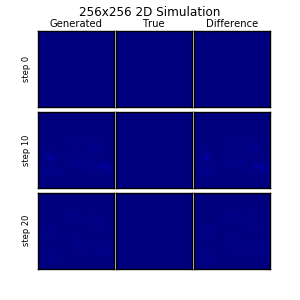
\includegraphics[scale=0.151]{../test/figs/256x256_2d_flow_image.png}}
\subfigure{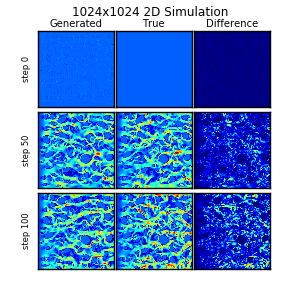
\includegraphics[scale=0.151]{../test/figs/1024x1024_2d_flow_image.png}}
\subfigure{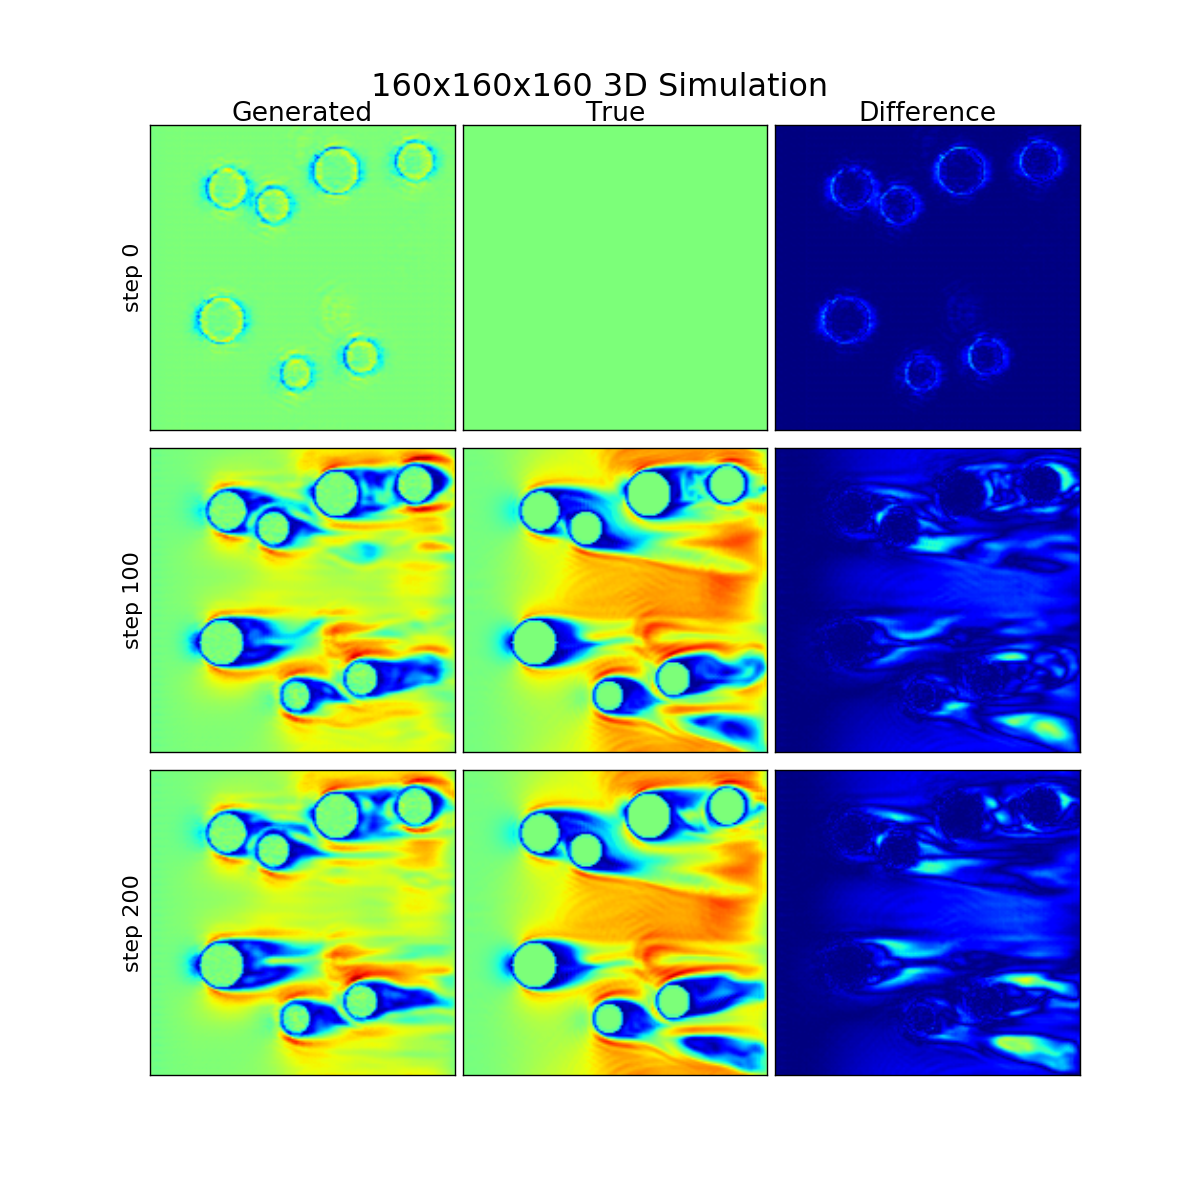
\includegraphics[scale=0.151]{../test/figs/160x160x160_3d_flow_image.png}}
\caption{A visual comparison of flows generated by Lat-Net and the Lattice Boltzmann method. Each figure shows the Generated, True, and Difference of the flow for various time steps.}
\label{2d_image_plot}
\end{figure}

\begin{figure}[!t]
\centering
\subfigure{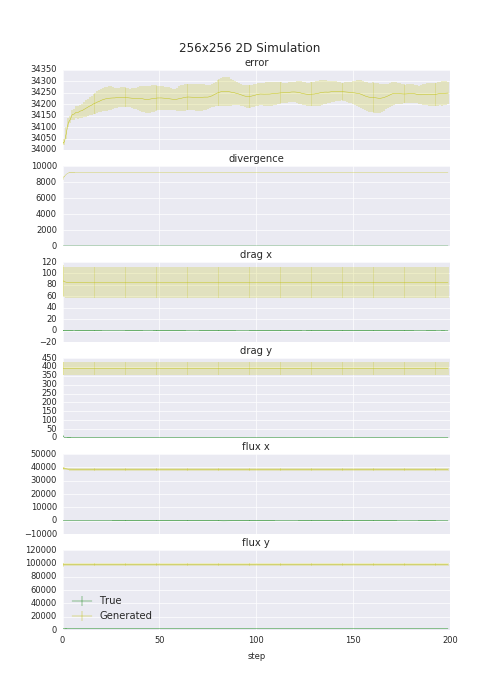
\includegraphics[scale=0.280]{../test/figs/256x256_2d_error_plot.png}}
\subfigure{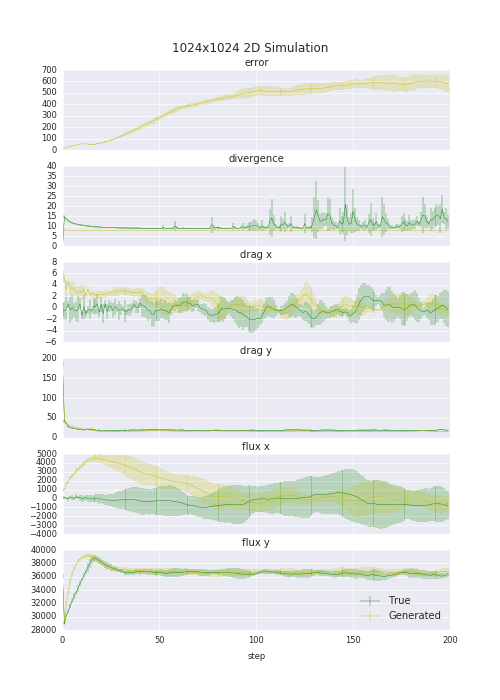
\includegraphics[scale=0.280]{../test/figs/1024x1024_2d_error_plot.png}}
\subfigure{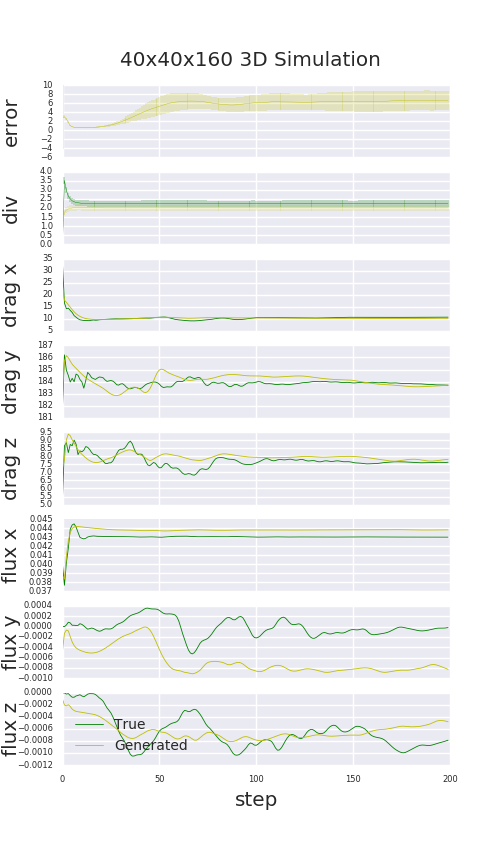
\includegraphics[scale=0.280]{../test/figs/40x40x160_3d_error_plot.png}}
\subfigure{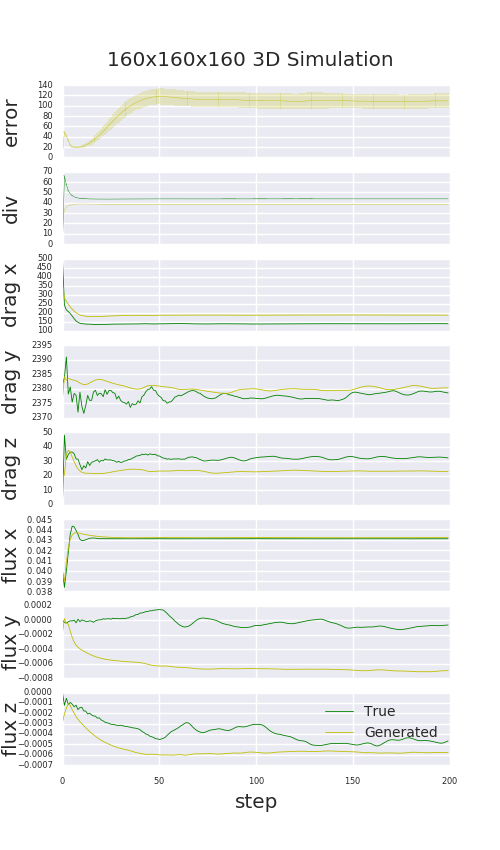
\includegraphics[scale=0.280]{../test/figs/160x160x160_3d_error_plot.png}}
\caption{ Comparison plot of the flows generated by Lat-Net and the Lattice Boltzmann method. Each plot shows the average mean squared error of the true and generated generated along with the average divergence of the velocity vector field for both simulations. The standard diviation is also displyed. In addition, the calclulated values for drag and flux are displayed for a single simulation.}
\label{2d_error_plot}
\end{figure}

\begin{figure}[!t]
\centering
\subfigure{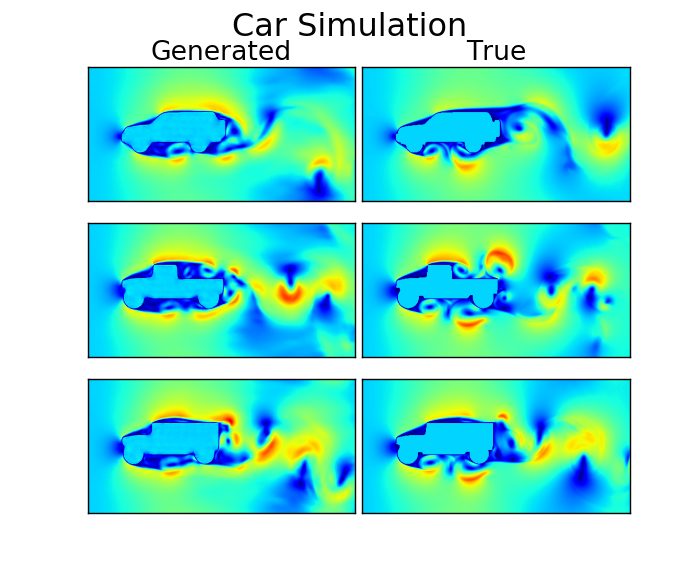
\includegraphics[scale=0.4]{../test/figs/car_2d_flow_image.png}}
\subfigure{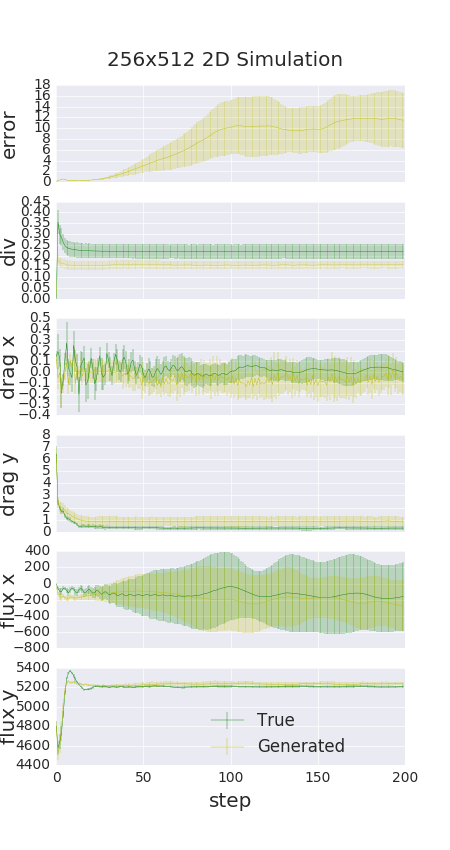
\includegraphics[scale=0.3]{../test/figs/256x512_2d_error_plot.png}}
\caption{Comparison of generated flows for the vehical cross section dataset. The images show the generated and true flow at step 100 for 3 different cars in the dataset. The plot shows the same values as described in \ref{2d_error_plot}.}
\label{car_dataset}
\end{figure}


A key componet of our model is its ability to generate larger simulations then those trained on. To test its effectiveness in doing so, we generate various sized 2D and 3D simulations and compare accuracy to ground truth simulations.

Comparing the accuracy of our simulations require some consideration. The simplest approach is to compare the MSE between the generated and true simulation at various timesteps. The problem with this approach is that fluid flow is a chaotic dynamical system and small perdibations in flow quickley compound leading to dramatic diffrences. For this reason, we compare a variety of metrics in evaluating the generated flows accuracy. Similar to \cite{tompson2016accelerating}, we compare the divergence of the generated and true velocity vector field. These values should be small (need to come back to this). We also compare the computed values of drag and flux from the simulation. Flow simulations are often run to calculate such values so comparing this is a strong indecator of our models real world applicability. The drag is calculated directly from the lattice state via the momentum transfer method \cite{guo2013lattice}. The flux value is the average of the flux in each non boundary cell. These values can be used to calculate important quantities such as drag coefiencet and reynolds number. Lastley, we visualy inspect the produced flow to check for instabilityes and bluring effects.

In figure \ref{2d_error_plot} we see the predicted values averaged over the test set of simulations along with the standard deviation. We also see that in the 2D simulations, Lat-Net is able to effectively transfer to larger domain sizes with similar calculated values of drag and flux. We also see that while our 3D model tends to have a bias in predicting (need actual figs).

When visually inspecting our produced flows (figure \ref{2d_image_plot}), we see a slight blurring effect but overal similar structure. We attribute this blur effect to the use of MSE loss. This can possibly be overcome with the use of generative advesarial network \cite{goodfellow2014generative} where the loss is derived from a discriminator network. Another solution may be to craft a loss function that takes advantage of the statistical properties of fluid flow such as the (I will leave blank for now) \cite{kim2008wavelet}. We leave these pursutes to future work.

The boundarys used in the above evaluation are drawn from the same distrobution as the train set. This motivates the question of how our model performs on drasticly different geometries. To test this, we apply our model to predicting flow around vehical cross sections. Supprisingly, even though are model is only trained on flows around simple shapes (ovals and rectangles) it can effectively generalize to this distinctly different dataset. In figure \ref{car_dataset}, we see the predicted flows are quite similar but with the same bluring effect. Calculating the same values seen above, we notice blaa.


\subsection{Computational Speed Up}

\begin{table}[]
\small
\caption{Computation time of Networks peices} \label{compute_times}
\centering
\begin{tabular}{|l|llllll|}
\hline
Simulation    & Comp. Factor       & Comp. Mapping       & Full State  & Plane      & Line       & Point \\ \hline
(1024, 1024)  & 18                 & 2.70 ms            & 36.24 ms   & na         & 6.71 ms   & 6.59 ms \\
(160, 160, 160) & 15                 & 23.05 ms           & 272.09 ms  & 38.20 ms  & 25.64 ms  & 24.06 ms  
\\ \hline
\end{tabular}
\label{computation_table}
\end{table}


In this section we investigate the computational speed up of our model. The standard performance metric for Lattice Boltzmann Codes is Million Lattice Updates per Second (MLUPs). This metric is calculated by the following equation,
\begin{equation}
  MLUP = \frac{n_x \times n_y \times n_z \times 10^{-6}}{Compute \ Time}
\end{equation}
 where $n_x$, $n_y$, and $n_z$ are the dimenstions of the simulation. For 3 dimensitonal simulations like the ones seen in this paper, a speed of 1,200 MLUPS can be achieved with a Nvidia K20 GPU and single percision floats \cite{januszewski2014sailfish}. We use this as our benchmark value to compare agianst.

The computation time and memory usage of the encoder can be neglected because this is a one time cost for the simulation. In addition, if the simulation is started with uniformly initialized flow as seen in our experiments, the computation to compress the flow is extremely redudent and can easily be optimized.

As seen in table \ref{computation_table}, the computation time of the compression mapping is shown to be 23.1 ms for a 3D simulation of grid size 160 by 160 by 160. Because each step of the compression mapping is equevilent to 60 lattice boltzmann steps, this equates to 10,600 MLUPS and a roughly 10x speed increase (a similar speedup is seen with the 2D simulation). This does not give a complete picture though. Once the compressed states have been generated, the generated flow must be extracted with the decoder. Unforcunatly, this requires considerable amounts of computation and memory because it involves applying convolutions to the full state size. Forcunatly, there are ways around this. In many applications of CFD, it is not nesicary to to have the full state information of the flow at each time step. For example, calculating the drag only requires integrating over the surface of the object. By using the convolutional nature of the decoder, we can extract spesicif pieces of the flow out without needing to extract the full state. In table \ref{computation_table} we show computation times for exracting out the flow information of a plane, line and single point in the 3D simulation. While these computations can still be somewhat expensive, they do not nececarly need to be performed at every time step and require very little working memory. 

Regretably, there are some measurements that do require the full state information to compute such as the average flux seen in our tests. Our current method is currently unable to handle these in its current form without requiring high runtimes and large working memory. A possible solution to this is training a seperate neural network that takes in the compressed state and predicts the desired measurement such as flux. This would negate the need to extract out the full state and keep memory usage low. We leave this and similar ideas for future work.

%While Lat-Net does compress the simulation state size by more then an order of magnetude, the working memory requirements for the compression network can be considerable. We have absurved

\subsection{Memory Compression}

\begin{wrapfigure}{R}{0.5\textwidth}
  \centering
  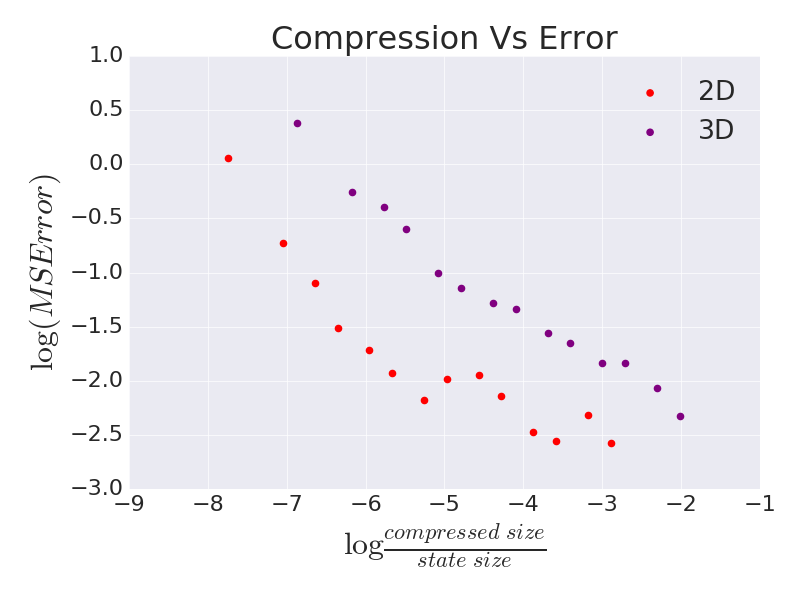
\includegraphics[scale=0.3]{../test/figs/compression_error_plot.png}
  \caption{This figure shows the trade off  of compression and error for 2D and 3D flows. The axis are put on a log scale to better display this trade off.}
  \label{compression_plot}
\end{wrapfigure}

One of the main purposes of Lat-Net is to compress the memory requirement of large simulations and so it is a natural question to ask what effect the compression has on error. The ideal method to test this would be to train many models with different compression ratios and compare their accuracy. Unforcunatly, training models is extremely computational intensive and so we propose another approach. We instead train $\phi_{enc}$ and $\phi_{dec}$ in an autoencoder fassion and then measure the reconsturction MSE on the test set. This less computationaly expensive approach allows many models to be trained and evaluated.

By keeping the architeture of $\phi_{enc}$ and $\phi_{dec}$ the same and vareing the final compressed filter size we see the trade off between compression and error. The results of this can be seen in figure \ref{compression_plot}. It is interesting to see a slight diminising return effect for low compression ratios. In chosing a network architeture for Lat-Net, there is always a trade off between compression and error. By plotting corrilation we have demostrated an effective tool picking a network with the desired trade off.

\subsection{Electromagnetic Results}

Finally, we illustrate the generatlity of our method by applying it to electromagnetic simulations. The same nueral network architecture is used as in the 2D flow simulations with the only difference being the filter size on the compression is half of that in the flow network. The loss is kept identical however the lattice values are scaled up by a factor of 10 so they are on the same scale as the flow lattice values. In figure \ref{em_dataset} we see that. We see that once the network is trained, it can readily be applied to larger simulations.

\begin{figure}[!t]
\centering
\subfigure{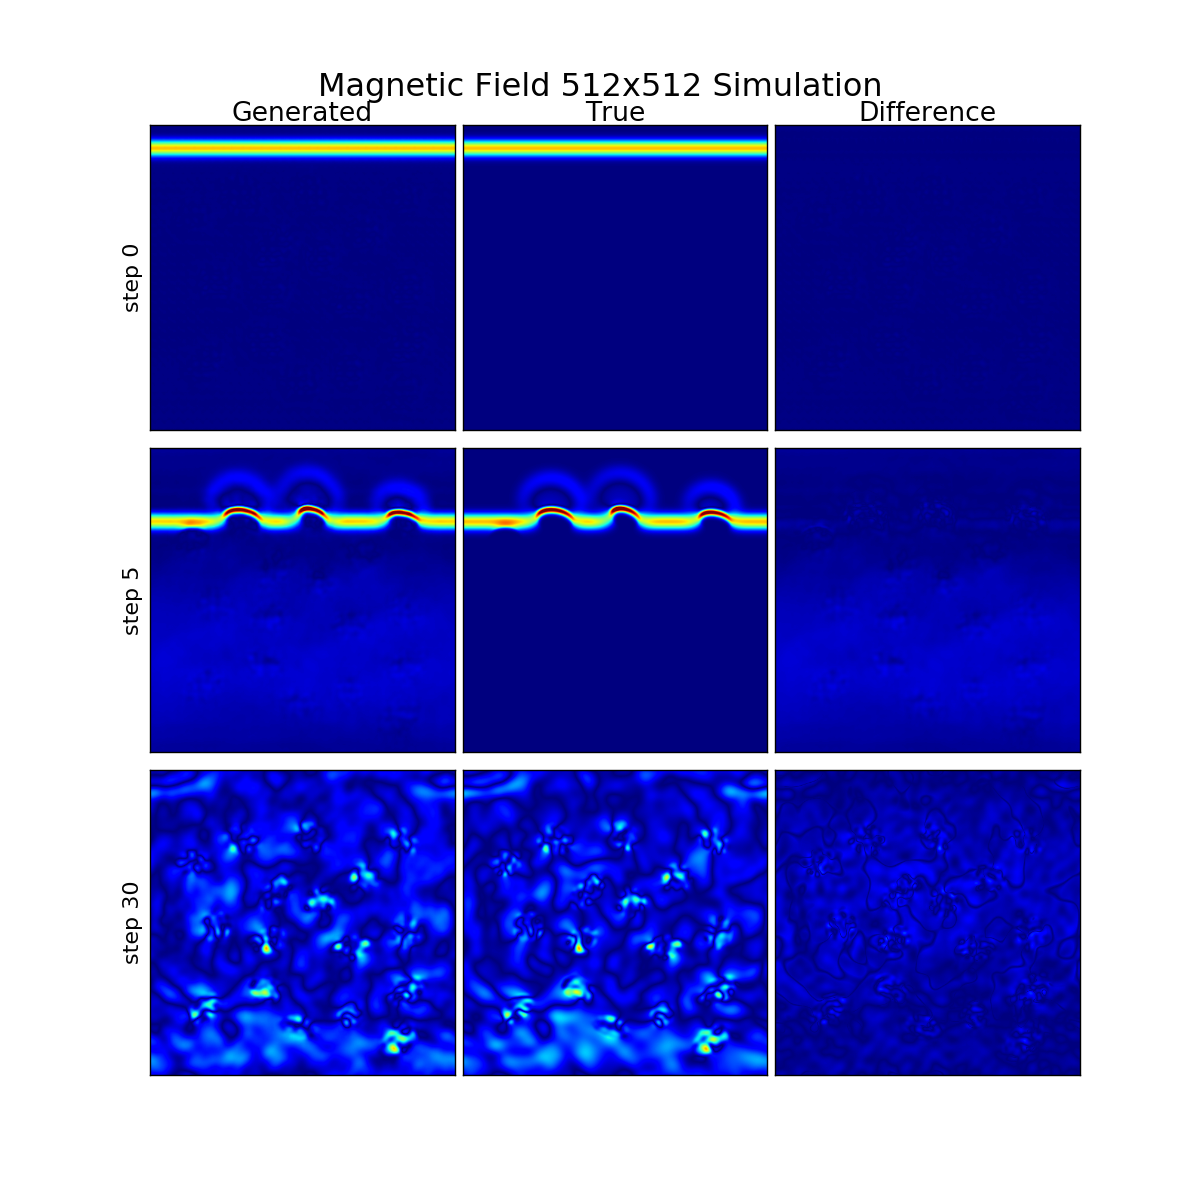
\includegraphics[scale=0.15]{../test/figs/512x512_2d_em_image.png}}
\subfigure{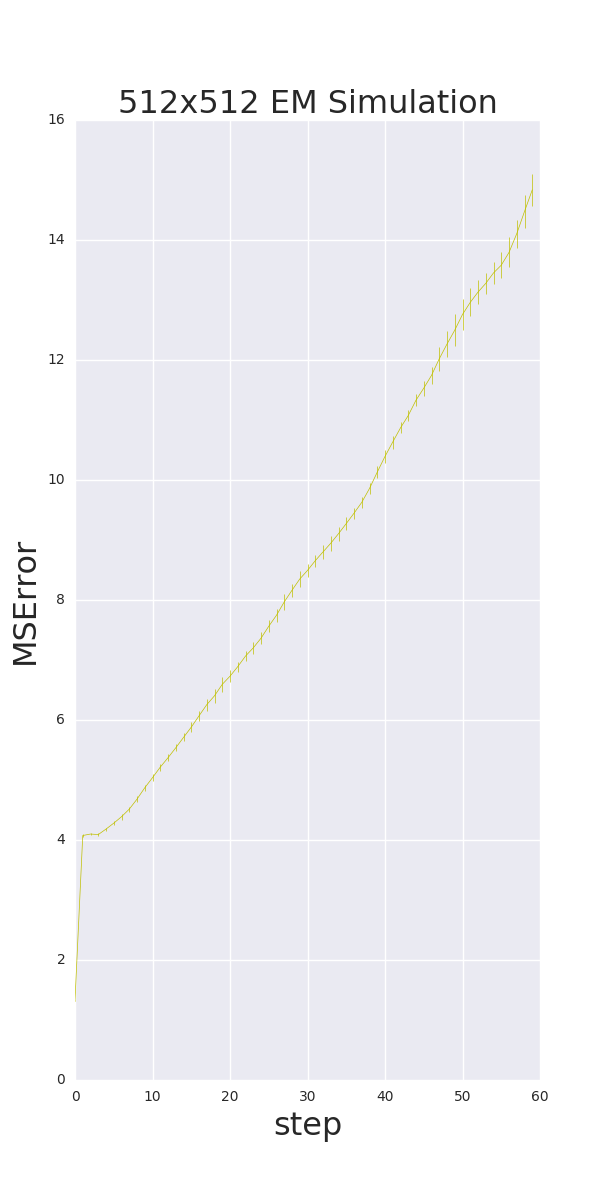
\includegraphics[scale=0.15]{../test/figs/512x512_2d_em_error_plot.png}}
\caption{ Comparison of generated Electromagnetic fields. The images show the true and generated magnetic field a various time steps. The reflection and refraction phemonomeo can clearly be seen in both as the electromagnetic wave interacts with objects of different dielectric constants. The plot shows the mean squared error of the true and generated simulation.}
\label{em_dataset}
\end{figure}


\section{Conclusion}

Fluid Simulations are increadbly important for a variety of tasks however they are extreamely computation and memory intensive. In this work we have developed a unique method to overcome this using deep neural networks. We have demonstrated it is capable of accuratly reconstructing a variety of simulations under different conditions with significantly less computation and memory. We have also shown that our method can be readly applied to other physics simulations such as electromagnetic simulations. While our method has proved succesful on the problems in this paper, there is still significant room for improvment. A loss function that either takes into account the statistical nature of the flow or uses recent advances in GANs could produce shaper more realistic flow. Training a network to extract desired measurements from the compressed state such as average flux would overcome the current memory limitation for such a task. We leave these and other improvements for future work.

\bibliography{references}
\bibliographystyle{ieeetr}

\end{document}
